\documentclass[12pt,]{article}
\usepackage{lmodern}
\usepackage{amssymb,amsmath}
\usepackage{ifxetex,ifluatex}
\usepackage{fixltx2e} % provides \textsubscript
\ifnum 0\ifxetex 1\fi\ifluatex 1\fi=0 % if pdftex
  \usepackage[T1]{fontenc}
  \usepackage[utf8]{inputenc}
\else % if luatex or xelatex
  \ifxetex
    \usepackage{mathspec}
  \else
    \usepackage{fontspec}
  \fi
  \defaultfontfeatures{Ligatures=TeX,Scale=MatchLowercase}
\fi
% use upquote if available, for straight quotes in verbatim environments
\IfFileExists{upquote.sty}{\usepackage{upquote}}{}
% use microtype if available
\IfFileExists{microtype.sty}{%
\usepackage{microtype}
\UseMicrotypeSet[protrusion]{basicmath} % disable protrusion for tt fonts
}{}
\usepackage[margin=1in]{geometry}
\usepackage{hyperref}
\PassOptionsToPackage{usenames,dvipsnames}{color} % color is loaded by hyperref
\hypersetup{unicode=true,
            pdftitle={LR Theory},
            pdfauthor={Tim Radtke},
            colorlinks=true,
            linkcolor=Maroon,
            citecolor=Blue,
            urlcolor=blue,
            breaklinks=true}
\urlstyle{same}  % don't use monospace font for urls
\usepackage{graphicx,grffile}
\makeatletter
\def\maxwidth{\ifdim\Gin@nat@width>\linewidth\linewidth\else\Gin@nat@width\fi}
\def\maxheight{\ifdim\Gin@nat@height>\textheight\textheight\else\Gin@nat@height\fi}
\makeatother
% Scale images if necessary, so that they will not overflow the page
% margins by default, and it is still possible to overwrite the defaults
% using explicit options in \includegraphics[width, height, ...]{}
\setkeys{Gin}{width=\maxwidth,height=\maxheight,keepaspectratio}
\IfFileExists{parskip.sty}{%
\usepackage{parskip}
}{% else
\setlength{\parindent}{0pt}
\setlength{\parskip}{6pt plus 2pt minus 1pt}
}
\setlength{\emergencystretch}{3em}  % prevent overfull lines
\providecommand{\tightlist}{%
  \setlength{\itemsep}{0pt}\setlength{\parskip}{0pt}}
\setcounter{secnumdepth}{5}
% Redefines (sub)paragraphs to behave more like sections
\ifx\paragraph\undefined\else
\let\oldparagraph\paragraph
\renewcommand{\paragraph}[1]{\oldparagraph{#1}\mbox{}}
\fi
\ifx\subparagraph\undefined\else
\let\oldsubparagraph\subparagraph
\renewcommand{\subparagraph}[1]{\oldsubparagraph{#1}\mbox{}}
\fi

%%% Use protect on footnotes to avoid problems with footnotes in titles
\let\rmarkdownfootnote\footnote%
\def\footnote{\protect\rmarkdownfootnote}

%%% Change title format to be more compact
\usepackage{titling}

% Create subtitle command for use in maketitle
\newcommand{\subtitle}[1]{
  \posttitle{
    \begin{center}\large#1\end{center}
    }
}

\setlength{\droptitle}{-2em}
  \title{LR Theory}
  \pretitle{\vspace{\droptitle}\centering\huge}
  \posttitle{\par}
  \author{Tim Radtke}
  \preauthor{\centering\large\emph}
  \postauthor{\par}
  \date{}
  \predate{}\postdate{}

\usepackage[retainorgcmds]{IEEEtrantools}
\usepackage{bm}
\usepackage{amsmath}
\usepackage{bbm}
\newtheorem{theorem}{Theorem}
\newtheorem{lemma}{Lemma}
\newcommand{\KL}{\,\text{KL}}
\newcommand{\der}{\,\text{d}}

\begin{document}
\maketitle

\section{Kullback-Leibler Divergence
Strategy}\label{kullback-leibler-divergence-strategy}

We start with a definition of the Likelihood Ratio. See for example
Example 6 in \url{http://math.arizona.edu/~jwatkins/s-lrt.pdf}.

In our strategy, we will have at time \(t\) a sample of observations for
arm \(i\) of size \(T_i(t)\): \(X = x_1, ..., x_{T_i(t)}\). Since we are
only considering Bernoulli distributions at this point, the Likelihood
for a sample from distribution \(Ber(\mu)\) is given by

\[ 
L(\mu|X) = (1-\mu)^{T_i(t) - \sum_{s = 1}^{T_i(t)} x_s} \mu^{\sum_{s = 1}^{T_i(t)} x_s}
\]

We want to test whether the sample \(X\) with maximum likelihood
estimate (\(H_1: \mu = \hat{\mu}\)) is actually different from the
standard hypothesis that it is equal to the threshold \(\tau\)
(\(H_0: \mu = \tau\)). To test this, we can use the likelihood ratio:

\[
\Lambda = \frac{L(\tau|X)}{L(\hat{\mu}|X)} = \frac{\tau^{\hat{\mu}T_i(t)}(1-\tau)^{(1-\hat{\mu})T_i(t)} }{\hat{\mu}^{\hat{\mu}T_i(t)}(1-\hat{\mu})^{(1-\hat{\mu})T_i(t)}}
\]

If the likelihood ratio is large, then it's quite likely that the sample
was generated by a Bernoulli distribution with parameter \(\tau\). If
the ratio is small, then the maximum likelihood estimate is very
different from the threshold. The statistic should be smaller than 1
given that we compare to the maximum likelihood estimate.

In an adaptive sampling strategy that is based on this ratio, it is
natural to pull the arm that currently maximizes the ratio (an arm with
distribution close to \(\tau\)). Even if the true parameter \(\mu\) is
close to \(\tau\), the ratio will increase over time as \(T_i(t)\)
increases. Thus given two distributions with the same maximum likelihood
estimate, the strategy will pull the arm that has a smaller \(T_i(t)\).

Thus our strategy could be to pull arm \(i^*\) at time \(t+1\) that
maximizes \(\tilde{B}_i(t) = \Lambda_i\). Of course,
\(\arg \max_i \Lambda_i(t) = \arg \min_i -\log(\Lambda_i(t))\). And so
an equivalent strategy is to pull
\(i^*(t) = \arg \min_i -\log(\Lambda_i(t))\). We now show that this is
equivalent to \(i^*(t) = \arg \min_i T_i(t)\hat{\KL}(\hat{\mu}||\tau)\).

We have

\begin{align*}
-\log(\Lambda_i(t)) & = \hat{\mu}T_i(t) \log(\frac{\hat{\mu}_i(t)}{\tau}) + (1-\hat{\mu})T_i(t) \log(\frac{1-\hat{\mu}_i(t)}{1-\tau}) \\
& = T_i(t) [\hat{\mu}_i(t) \log(\frac{\hat{\mu}_i(t)}{\tau}) + (1-\hat{\mu}_i(t)) \log(\frac{1-\hat{\mu}_i(t)}{1-\tau})] \\
& = T_i(t) \der(\hat{\mu}_i(t), \tau) \\
& = B_i(t)
\end{align*}

This notation of the index will prove useful in theoretical derivations,
while the likelihood ratio is advantageous in the implementation of the
algorithm, as it can be computed even when \(\hat{\mu}=0\) or
\(\hat{\mu}=1\), which will always occur in the beginning of the
sampling.

\subsection{Comparison with Other
Indices}\label{comparison-with-other-indices}

If we consider \(B_i^{KL}(t) = T_i(t) \der(\hat{\mu}_i(t), \tau)\), we
see a similarity to the index that first showed up in Locatelli et al.
(2016) with the APT strategy where
\(B^{APT}_i(t) = \sqrt{T_i(t)} \Delta_i(t) = \sqrt{T_i(t)} |\mu_i(t) - \tau|\)
(if we consider the case where \(\epsilon = 0\)). This format for the
strategy's index was inherited by
\href{https://arxiv.org/pdf/1704.04567.pdf}{Zhong et al. (2017)} for
their EVT algorithm which adapts both the term estimating the difference
between \(\hat{\mu}\) and \(\tau\), which I will now refer to as
\(D_k(t)\), and the confidence term of the current estimate, which they
call \(S_i^{EVT}(t)\). In Zhong et al., the index is given by
\(B_i^{EVT}(t) = D_i^{EVT}(t)S^{EVT}_i(t)\), where the difference term
\(D_i^{EVT}(t) = D_i^{APT}(t) = |\mu_i(t) - \tau|\), but where the
confidence term \(S_i^{EVT}(t)\) is no longer equal to
\(S_i^{APT}(t)=\sqrt{T_i(t)}\) but
\(S_i^{EVT}(t) = \Big(\frac{a}{T_i(t)} + \sqrt{\frac{a}{T_i(t)}}\hat{\sigma}_i(t)\Big)\),
and thus depends on the current estimate of the variance,
\(\hat{\sigma}_i(t)\). Continuing this format of indices, the strategy
proposed above has an index that can be written as

\[
B_i(t) = S^{KL}_i(t) D_i^{KL}(t) = T_i(t) \der(\hat{\mu}_i(t), \tau)
\]

If we write the Kullback-Leibler divergence as approximated by a Normal
distribution,
\(\der(\hat{\mu}, \tau) \approx \frac{(\hat{\mu}-\tau)^2}{\tau(1-\tau)}\)
or using Pinsker's inequality to bound it as
\(\der(\hat{\mu}, \tau) \geq 2|\hat{\mu}-\tau|^2\), we see that these
approximations lead to the index that is used by the APT strategy. Thus,
the motivation behind the likelihood ratio based strategy is to improve
upon APT for cases where the approximation fails. We see that in the
case of Bernoulli distributions, the two strategies are equivalent for
\(\tau = 0.5\).

\subsection{Upper Bound for KL
Strategy}\label{upper-bound-for-kl-strategy}

Given the general schema for the index in both the APT and the EVT
strategy, the proofs for their respective upper bound on the expected
loss share certain steps. Both proofs build on favorable events which
hold with large probability for certain levels of \(T\), \(T_i\), \(H\).
In both proofs, the authors bound the number of pulls that a helpful arm
receives; that is, an arm that received at least a share of the budget
\(T\) that is proportional to his contribution to the overall complexity
\(H\), and which is played in the final round \(T\). Both strategies
need to show that on the favorable event, after \(T\) rounds, every arm
has been pulled a suffient amount of times for \(\hat{\mu}_i(T)\) to be
seperated sufficiently from \(\tau\) to make a correct classification of
arm \(i\). In the design of the favorable event, both strategies can use
the fact that the \(|\hat{\mu} - \tau|\) term in the index get the
following upper bound
\(|\hat{\Delta}_i(t) - \Delta_i| \leq |\hat{\mu}_i(t)-\mu_i|\) on the
\(D_i^{APT}(t) = D_i^{EVT}(t) = \hat{\Delta}_i(t)\) part of the index.
Given this bound, both proofs use a favorable event on which
\(\hat{\mu}\) is very close to \(\mu\) with large probability.

Given that the Kullback-Leibler divergence is not a metric, and more
specifically, the triangle inequality does not hold, the favorable event
from the other proofs will not suffice to bound \(D_i^{KL}(t)\).

Given the lower bound on \(T_k(t)\) for the helpful arm \(k\), and the
lower and upper bound on \(\hat{\Delta}_k(t)\) and \(\hat{\Delta}_i(t)\)
through the favorable event (compare equation (10) in A.2 of Locatelli
et al., 2016), all that remains to show the sufficiently seperated
\(\hat{\mu}\) from \(\tau\) is to lower bound the number of times the
not helpful arms are pulled, \(T_i(t)\). Locatelli et al. can derive
this easily from the other bounds by comparing the two indices
\(B_k(t)\) and \(B_i(t)\). Since at time \(t\) the arm \(k\) has been
pulled, the APT strategy has \(B_k^{APT}(t) \leq B_i^{APT}(t)\), since
the algorithm pulls the \(\arg \min\). Similar holds for the EVT
algorithm. And using the Kullback-Leibler distance instead of the
Likelihood-ratio, the KL based strategy also minimizes \(B_i(t)\)
(instead of maximizing \(\tilde{B}_i(t)\).

Thus, for the KL-based strategy, consider again for the helpful arm
\(k\) pulled at time \(t\), and some other arm \(i\):

\[
B_k(t) \leq B_i(t) \Leftrightarrow T_k(t) \der(\hat{\mu}_k(t), \tau) \leq T_i(t) \der(\hat{\mu}_i(t), \tau)
\]

Starting from here, our goal will be to show that some kind of
seperation of the arms holds on the favorable event, where the favorable
event is set up such that the above quantities are bounded and the
seperation condition can be checked. On the way, the favorable event
will have an impact on how the complexity \(H\) will be defined for this
problem. In the end, we want to derive an upper bound of rate
\(\exp(-\frac{T}{H})\) on the error probability.

To achieve correct seperation at the end of the algorithm,
\href{https://arxiv.org/pdf/1704.04567.pdf}{Zhong et al. (2017)} require
that after the last round \(T\), the sample means \(\hat{\mu}\) of the
arms are closer to the true mean \(\mu\) of the distribution than to the
threshold \(\tau\):

\[
|\hat{\mu}_i(T_i(T)) - \mu| \leq \frac{\Delta_i}{2}
\]

More explicitly, for an arm below the threshold, \(\mu_i < \tau\), they
demand \(\hat{\mu}_i(T_i(T)) \geq \mu_i - \frac{\mu_i-\tau}{2}\). On the
other hand, for an arm above the threshold, \(\mu_i \geq \tau\), they
demand \(\hat{\mu}_i(T_i(T)) \leq \mu_i - \frac{\mu_i-\tau}{2}\).

Based on a similar idea, the fixed-confidence KL-LUCB algorithm
introduced in
\href{http://proceedings.mlr.press/v30/Kaufmann13.pdf}{Kaufmann and
Kalyanakrishnan} (2013) for the Top-\(m\) problem employs a stopping
rule that checks whether the smallest lower bound among the currently
best \(m\) algorithms is larger than the largest upper bound of the
other arms that currently are not among the \(m\) best. If the lower
bound is larger than the upper bound, the two sets of arms are
considered to be sufficiently seperated; it is unlikely, that there are
two arms that are classified into the wrong set (compare with
Proposition 1,
\href{http://proceedings.mlr.press/v30/Kaufmann13.pdf}{Kaufmann and
Kalyanakrishnan}, 2013).

Thus a simple demand that we can pose for our strategy is the one from
Zhong et al. (2017), which directly translates into

\[
\der(\hat{\mu}_i(T_i(T)), \tau) \geq \der(\mu_i +\frac{\tau-\mu_i}{2}, \tau)
\]

for arms with mean below the threshold, \(\mu_i < \tau\). On the other
hand, for arms with mean above the threshold, \(\mu_i > \tau\), we
demand

\[
\der(\hat{\mu}_i(T_i(T)), \tau) \geq \der(\mu_i - \frac{\mu_i - \tau}{2}, \tau).
\]

These two conditions are equivalent to the conditions given in
\href{https://arxiv.org/pdf/1704.04567.pdf}{Zhong et al. (2017)} due to
the monotonicity of the KL divergence. If we could check whether these
conditions hold on whatever favorable event we use, that would be a very
convenient check.

UPDATE: This translation into the Kullback-Leibler distance does not
work as easily, because the above conditions might hold even if
\(\mu < \tau < \hat{\mu}\), for example.

\subsubsection{The Favorable Event}\label{the-favorable-event}

Intuitively, it should be an event of large probability that
\(|\der(\mu,\tau) - \der(\hat{\mu},\tau)|<\epsilon\), given that
\(|\mu - \hat{\mu}|<\delta\) is likely. Also since we know that
\(\der(\hat{\mu}(t), \mu) \leq \epsilon\) is likely for large \(t\)
following for example Proposition 1 in
\href{https://projecteuclid.org/download/pdfview_1/euclid.aos/1375362558}{Cappé
et al. (2013)}. Additionally we know that
\(\der(\hat{\mu}, \tau) = \der(\mu, \tau)\) for \(\hat{mu} = \mu\),
however otherwise the inequality
\(\der(\hat{\mu}, \tau) \geq \der(\hat{\mu}, \mu) + \der(\mu, \tau)\)
only holds for \(\mu \in [\hat{\mu}, \tau]\) (or
\(\mu \in [\tau, \hat{\mu}]\)).

Instead, we will try to base our favorable event on a variant of Lemma 1
in \href{http://proceedings.mlr.press/v30/Kaufmann13.pdf}{Kaufmann and
Kalyanakrishnan} (2013), which states the following.

Let \(T \geq 1\) be an integer. Let \(\delta > 0\), \(\gamma > 0\), and
\(c \in (0,1)\) be such that \(mu_a \neq \tau\).

\[
\sum_{t=1}^T \mathbb{P} \Big(a = u_t \lor a = l_t, T_a(t) > \left \lceil{\frac{\gamma}{d^*(\mu_a,\tau)}}\right \rceil, T_a(t) d(\hat{\mu}_a, \tau) \leq \gamma \Big) \leq \frac{exp(-\gamma)}{d^*(\mu_a, \tau)}
\]

Given Lemma 2 in the same paper, as well as the proof of Lemma 1 in
Appendix C of the paper (last inequality), the same bound should hold if
we write the event without the lower and upper bounds \(u_t\) and
\(l_t\) of arm \(a\):

\[
\sum_{t=1}^T \mathbb{P} \Big(T_a(t) > \left \lceil{\frac{\gamma}{d^*(\mu_a,\tau)}}\right \rceil, T_a(t) d(\hat{\mu}_a, \tau) \leq \gamma \Big) \leq \frac{exp(-\gamma)}{d^*(\mu_a, \tau)}
\]

Thus on the favorable event for a single arm \(a\), we have that

\[
T_a(t) -1 \geq \frac{\gamma}{d^*(\mu_a, \tau)} \qquad \text{and} \qquad d(\hat{\mu}_a, \tau) > \frac{\gamma}{T_a(t)}
\]

\subsubsection{Characterization of some helpful
arm}\label{characterization-of-some-helpful-arm}

Locatelli et al. (2016) show for arm \(k\) that
\(T_k(t) \geq T_k(T) - 1 \geq \frac{T}{2H_{APT}\Delta^2_{APT,k}}\). We
expect (CHECK THIS) that a similar condition holds for our algorithm,
however with a different \(H_{KL}\) and \(h_{KL,k}\),
\(H_{KL} = \sum_{i=1}^K h_{KL,i}\),
\(h_{APT,k} = 1/(|\hat{\mu}-\tau|+\epsilon)^2\); but where the helpful
arm \(k\) still has at least as many pulls as would be its share of the
budget given its contribution to the overall complexity.

Now, we can go ahead and plug the favorable event directly into
\(B_k(t)\) (on the favorable event, it is likely that
\(\gamma < T_a(t) d(\hat{\mu}_a, \tau)\)):

\[
B_k(t) \leq B_i(t) \Leftrightarrow \gamma < T_k(t) \der(\hat{\mu}_k(t), \tau) \leq T_i(t) \der(\hat{\mu}_i(t), \tau) 
\]

To check whether this makes sense, we need to choose a value for
\(\gamma\), such that the second part of the favorable event is
fulfilled. Given the lower bound for the helpful arm, we can define the
complexity in terms of the Chernoff information used in
\href{http://proceedings.mlr.press/v30/Kaufmann13.pdf}{Kaufmann and
Kalyanakrishnan} (2013). We write

\[
H_{KL} = \sum_{i=1}^K \frac{1}{d^*(\mu_i, \tau)}
\]

For two Bernoullis, the Chernoff information is defined as
\(d^*(\mu_i, \tau) = d(z^*,\mu_i) = d(z^*, \tau)\) (compare
\href{http://proceedings.mlr.press/v30/Kaufmann13.pdf}{Kaufmann and
Kalyanakrishnan}, 2013). For the helpful arm we thus get

\[
T_k(t) \geq T_k(T) -1 \geq \frac{T}{2 H_{KL} d^*(\mu_i, \tau)}
\] such that by choosing \(\gamma = \frac{T}{2H_{KL}}\) the favorable
event \(T_a(t) -1 > \frac{\gamma}{d^*(\mu_a, \tau)}\) works for the
helpful arm:

\[
\gamma = \frac{T}{2H_{KL}} \leq T_k(t) \der(\hat{\mu}_k(t), \tau) \leq T_i(t) \der(\hat{\mu}_i(t), \tau) 
\]

Given that we can conclude the proof successfully, this choice of the
exploration exponent \(\gamma\) already implies that the budget should
be rather large if \(H_{KL}\) is large. But it also implies that the
favorable event occurs at the rate that we demanded upfront, since then
\(exp(-\gamma) = exp(-T/(2H))\).

\subsubsection{Problem}\label{problem}

At this point, however, I am stuck since the favorable event does not
give an upper bound on the RHS of the equation. Thus I don't have a way
of bounding \(T_i(t)\). I tried to approximate the KL-divergence
\(d(\hat{\mu}_k(t), \tau) \leq \frac{(\hat{\mu}-\tau)^2}{\tau(1-\tau)}\)
to get a bound similarly as in Locatelli et al. (2016) using the
favorable event mentioned there; this gave me indeed a lower bound on
\(T_i(t)\) similar to the one in that paper. However, given that the
favorable event bounds the KL divergence from below as
\(\frac{\gamma}{T_a(t)} < d(\hat{\mu}_a, \tau)\), the lower bound for
\(T_i(t)\) did not prove useful. Instead, it might have showed me
another problem. At first I believed it would suffice to show that
\(d(\hat{\mu}_a, \tau)\) is larger than e.g. \(d^*(\mu_a, \tau)\) on the
favorable event. But in theory, this could also hold if \(\mu_a < \tau\)
and \(\tau < \hat{\mu}_a\). So a check against that probably needs to be
included in the favorable event as well. This might be possible with
some proposition from the
\href{https://projecteuclid.org/download/pdfview_1/euclid.aos/1375362558}{KL-UCB
paper by Cappé et al. (2013)}, or a self-normalized inequality by
\href{https://arxiv.org/pdf/1102.2490.pdf}{Garivier and Cappé (2011,
Theorem 10)}.

In general, I'm simply wondering which inequality might suffice to bound
\(B_k(t) < B_i(t)\). I believed that the one from
\href{http://proceedings.mlr.press/v30/Kaufmann13.pdf}{Kaufmann and
Kalyanakrishnan} sufficed, but in their paper it is combined with a nice
separation condition stemming from the lower and upper bounds, which is
integrated into the stopping rule of the fixed-\emph{confidence}
algorithm (where the separation thus has to hold).

\subsection{Experiments}\label{experiments}

First, we again show the result of experiment 3. This time around,
however, we set \(\epsilon = 0\) as recommended by Andrea. Also, we move
the two arms that previously have been inside the \(\epsilon\)-interval
a little away from the threshold \(\tau = 0.5\) to remove the need for a
very large sample size. The likelihood-ratio based algorithm is now able
to show it's advantage.

The setup is as follows:

\begin{verbatim}
##  [1] 0.001 0.005 0.010 0.015 0.040 0.060 0.085 0.090 0.095 0.099
\end{verbatim}

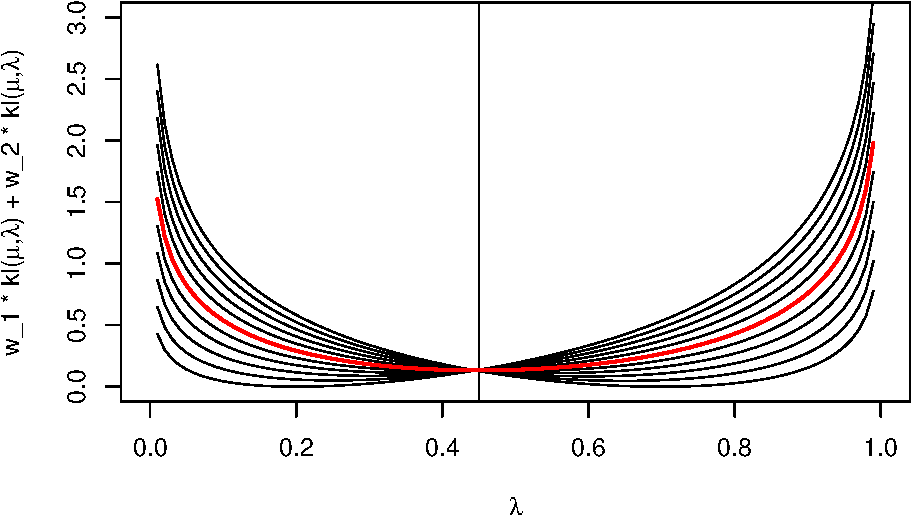
\includegraphics{LR_theory_files/figure-latex/unnamed-chunk-1-1.pdf}

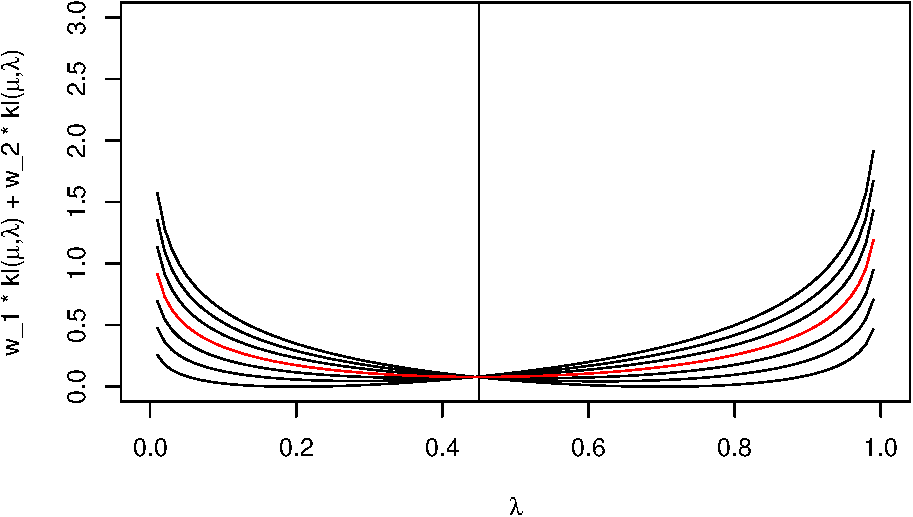
\includegraphics{LR_theory_files/figure-latex/unnamed-chunk-2-1.pdf}

\subsubsection{Experiment 2}\label{experiment-2}

This is a new setup in which the observations are set in more or less
the same distance from each other on a log10 scale. Again,
\(\epsilon = 0\). We choose a very small threshold with \(\tau = 0.01\).
Also note that we have increased the budget to \(T=10000\), while the
previous experiment had \(T=7000\).

\begin{verbatim}
##  [1] 0.00010 0.00032 0.00056 0.00100 0.00178 0.00316 0.00562 0.01413
##  [9] 0.01778 0.03162 0.10000
\end{verbatim}

\includegraphics{LR_theory_files/figure-latex/unnamed-chunk-3-1.pdf}

\includegraphics{LR_theory_files/figure-latex/unnamed-chunk-4-1.pdf}


\end{document}
